\documentclass{article}

\usepackage{ragged2e}
\usepackage{graphicx}
\usepackage{amsmath}
\usepackage{siunitx}

\begin{document}

\begin{flushright}
    \noindent
    Rodrigo Becerril Ferreyra\\
    CECS 211 Section 01\\
    Lab 6\\
    2019-10-22 to 2019-11-05
\end{flushright}

For this lab, we are tasked with solving a complex, multi-
sourced circuit using mesh analysis techniques. Here is the
circuit we will be solving\footnote{Note that this circuit has the mesh
currents added and labeled; the mesh loops do
not denote actual current.}:

\begin{figure}[h]
    \caption{Circuit with Mesh Loops}
    \centering
    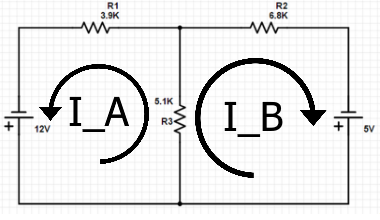
\includegraphics{Images/CircuitWithMeshCurrents.png}
\end{figure}

\section{Hand Calculations} As with any circuit, is is helpful
to calculate all theoretical values by hand before modeling
in a computer simulation or in real life, to have an idea
of what values one might expect. For mesh analysis, this is
done in several steps.

\subsection{Assigning Mesh Currents} Mesh currents can be assigned
arbitrarily; in this example, I've chosen to assign mesh
current \(I_A\) in a counter-clockwise fashion and current
\(I_B\) clockwise, as seen in
Figure 1.

\subsection{Writing KVL Equations} KVL tells us that the sum of
voltage drops in any closed loop must be equal to zero. In
mesh analysis, the KVL loops can be written with respect to 
the mesh loops. Starting from the top-right corner of loop
\(I_A\), its respective KVL expression is as follows:

\begin{align*}
    \SI{0}{\volt} &= (\SI{3.9}{\kilo\ohm}\cdot I_A) - \SI{12}{\volt} + (\SI{5.1}{\kilo\ohm}\cdot I_A) + ( \SI{5.1}{\kilo\ohm}\cdot I_B )\\
    \SI{12}{\volt} &= (\SI{9.0}{\kilo\ohm}\cdot I_A) + (\SI{5.1}{\kilo\ohm}\cdot I_B)
\end{align*}

Similarly, the KVL equation for \(I_B\) is as follows:

\begin{align*}
    \SI{0}{\volt} &= ( \SI{5.1}{\kilo\ohm}\cdot I_B ) - \SI{5}{\volt} + ( \SI{5.1}{\kilo\ohm} \cdot I_B ) + (\SI{5.1}{\kilo\ohm} \cdot I_A)\\
    \SI{5}{\volt} &= ( \SI{5.1}{\kilo\ohm}\cdot I_A ) + (\SI{11.9}{\kilo\ohm}\cdot I_B)
\end{align*}

To solve this system, we will use substitution; more
specifically, we will solve for \(I_B\) and use that to obtain \(I_A\).

Using the last equation:
\begin{align*}
    \SI{5}{\volt} &=  \SI{5.1}{\kilo\ohm}\cdot I_A  + \SI{11.9}{\kilo\ohm}\cdot I_B\\
    \SI{5.1}{\kilo\ohm}\cdot I_A &= \SI{5}{\volt} - \SI{11.9}{\kilo\ohm}\cdot I_B\\
    I_A &= \SI{0.980}{\milli\ampere} - 2.333I_B
\end{align*}

Plugging this value into the other equation, we have:
\begin{align*}
    \SI{9.0}{\kilo\ohm}\cdot I_A + \SI{5.1}{\kilo\ohm}\cdot I_B &= \SI{12}{\volt}\\
    \SI{9.0}{\kilo\ohm}\cdot (\SI{0.980}{\milli\ampere} - 2.333I_B) + \SI{5.1}{\kilo\ohm}\cdot I_B &= \SI{12}{\volt}\\
    \SI{8.82}{\volt} - \SI{20.997}{\kilo\ohm}\cdot I_B + \SI{5.1}{\kilo\ohm}\cdot I_B &= \SI{12}{\volt}\\
    \SI{-20.997}{\kilo\ohm}\cdot I_B + \SI{5.1}{\kilo\ohm}\cdot I_B &= \SI{3.18}{\volt}\\
    \SI{-15.897}{\kilo\ohm}\cdot I_B &= \SI{3.18}{\volt}\\
    I_B &= \SI{-0.200}{\milli\ampere}
\end{align*}

Using this value for \(I_B\), we can substitute back into the
equation to find the value for \(I_A\).
\begin{align*}
    I_A &= \SI{0.980}{\milli\ampere} - 2.333I_B\\
    I_A &= \SI{0.980}{\milli\ampere} - 2.333(\SI{-0.200}{\milli\ampere})\\
    I_A &= \SI{0.980}{\milli\ampere} + \SI{0.466}{\milli\ampere}\\
    I_A &= \SI{1.447}{\milli\ampere}
\end{align*}

Thus, our values for our mesh currents are
\(I_A = \SI{1.447}{\milli\ampere}\) and
\(I_B = \SI{-0.200}{\milli\ampere}\). Note that \(I_B\) is
negative, so the actual current goes the other way, in the
counter-clockwise direction.

\pagebreak

Our new mesh currents look like so:

\begin{figure}[h]
    \caption{New Mesh Loops}
    \centering
    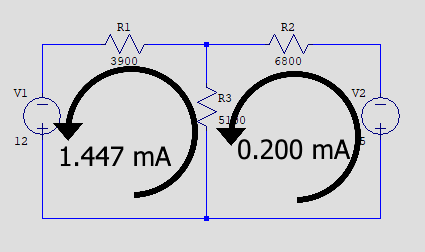
\includegraphics{Images/MeshCurrent.png}
\end{figure}

The current going through \(R_1\) and \(R_2\) are simple to
calculate, as there is only one current going through each.
However, \(I_{R_3}\) has two currents going through it.
The current on the left will prevail, however, because its
value is larger. The current arrows will look like so:

\begin{figure}[h]
    \caption{Current Arrows}
    \centering
    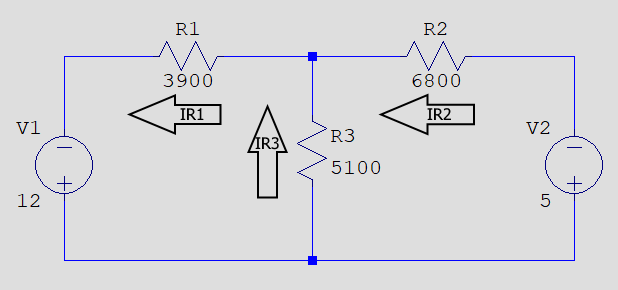
\includegraphics[width=\textwidth]{Images/RealCurrent.png}
\end{figure}

The value of \(I_{R_1}\) is \SI{1.447}{\milli\ampere} and the
the value of \(I_{R_2}\) is \SI{0.200}{\milli\ampere}.
The value of \(I_{R_3}\) is \(\SI{1.447}{\milli\ampere}
-\SI{0.200}{\milli\ampere} = \SI{1.247}{\milli\ampere}\).

\pagebreak

The voltage drop across the three resistors are as follows:
\(V_{R_1} = \SI{5.64}{\volt}\),
\(V_{R_2} = \SI{1.36}{\volt}\), and
\(V_{R_3} = \SI{6.36}{\volt}\).

There are three KVL equations in this circuit.
They are as follows (they all begin on the top-left corner
and go clockwise):
\begin{align*}
    \text{R1 to R3: }& -\SI{5.64}{\volt} - \SI{6.36}{\volt} + \SI{12}{\volt} &= 0\\
    \text{R2 to R3: }& -\SI{1.36} - \SI{5}{\volt} + \SI{6.36}{\volt} &= 0\\
    \text{R1 to R2: }& -\SI{5.64}{\volt} - \SI{1.36}{\volt} - \SI{5}{\volt} + \SI{12}{\volt} &= 0
\end{align*}

The next step was to recreate this circuit physically, on a
breadboard. We then measured the following values
for voltage: \(V_{R_1} = \SI{5.58}{\volt}\), \(V_{R_2} = \SI{1.31}{\volt}\),
and \(V_{R_3} = \SI{6.35}{\volt}\). The values for current are
as follows: \(I_{R_1} = \SI{1.42}{\milli\ampere}\),
\(I_{R_2} = \SI{0.19}{\milli\ampere}\), and
\(I_{R_3} = \SI{1.22}{mA}\).

The last step was to solder this circuit onto a perfboard.
After a brief training and safety course, our final product
turned out as so:

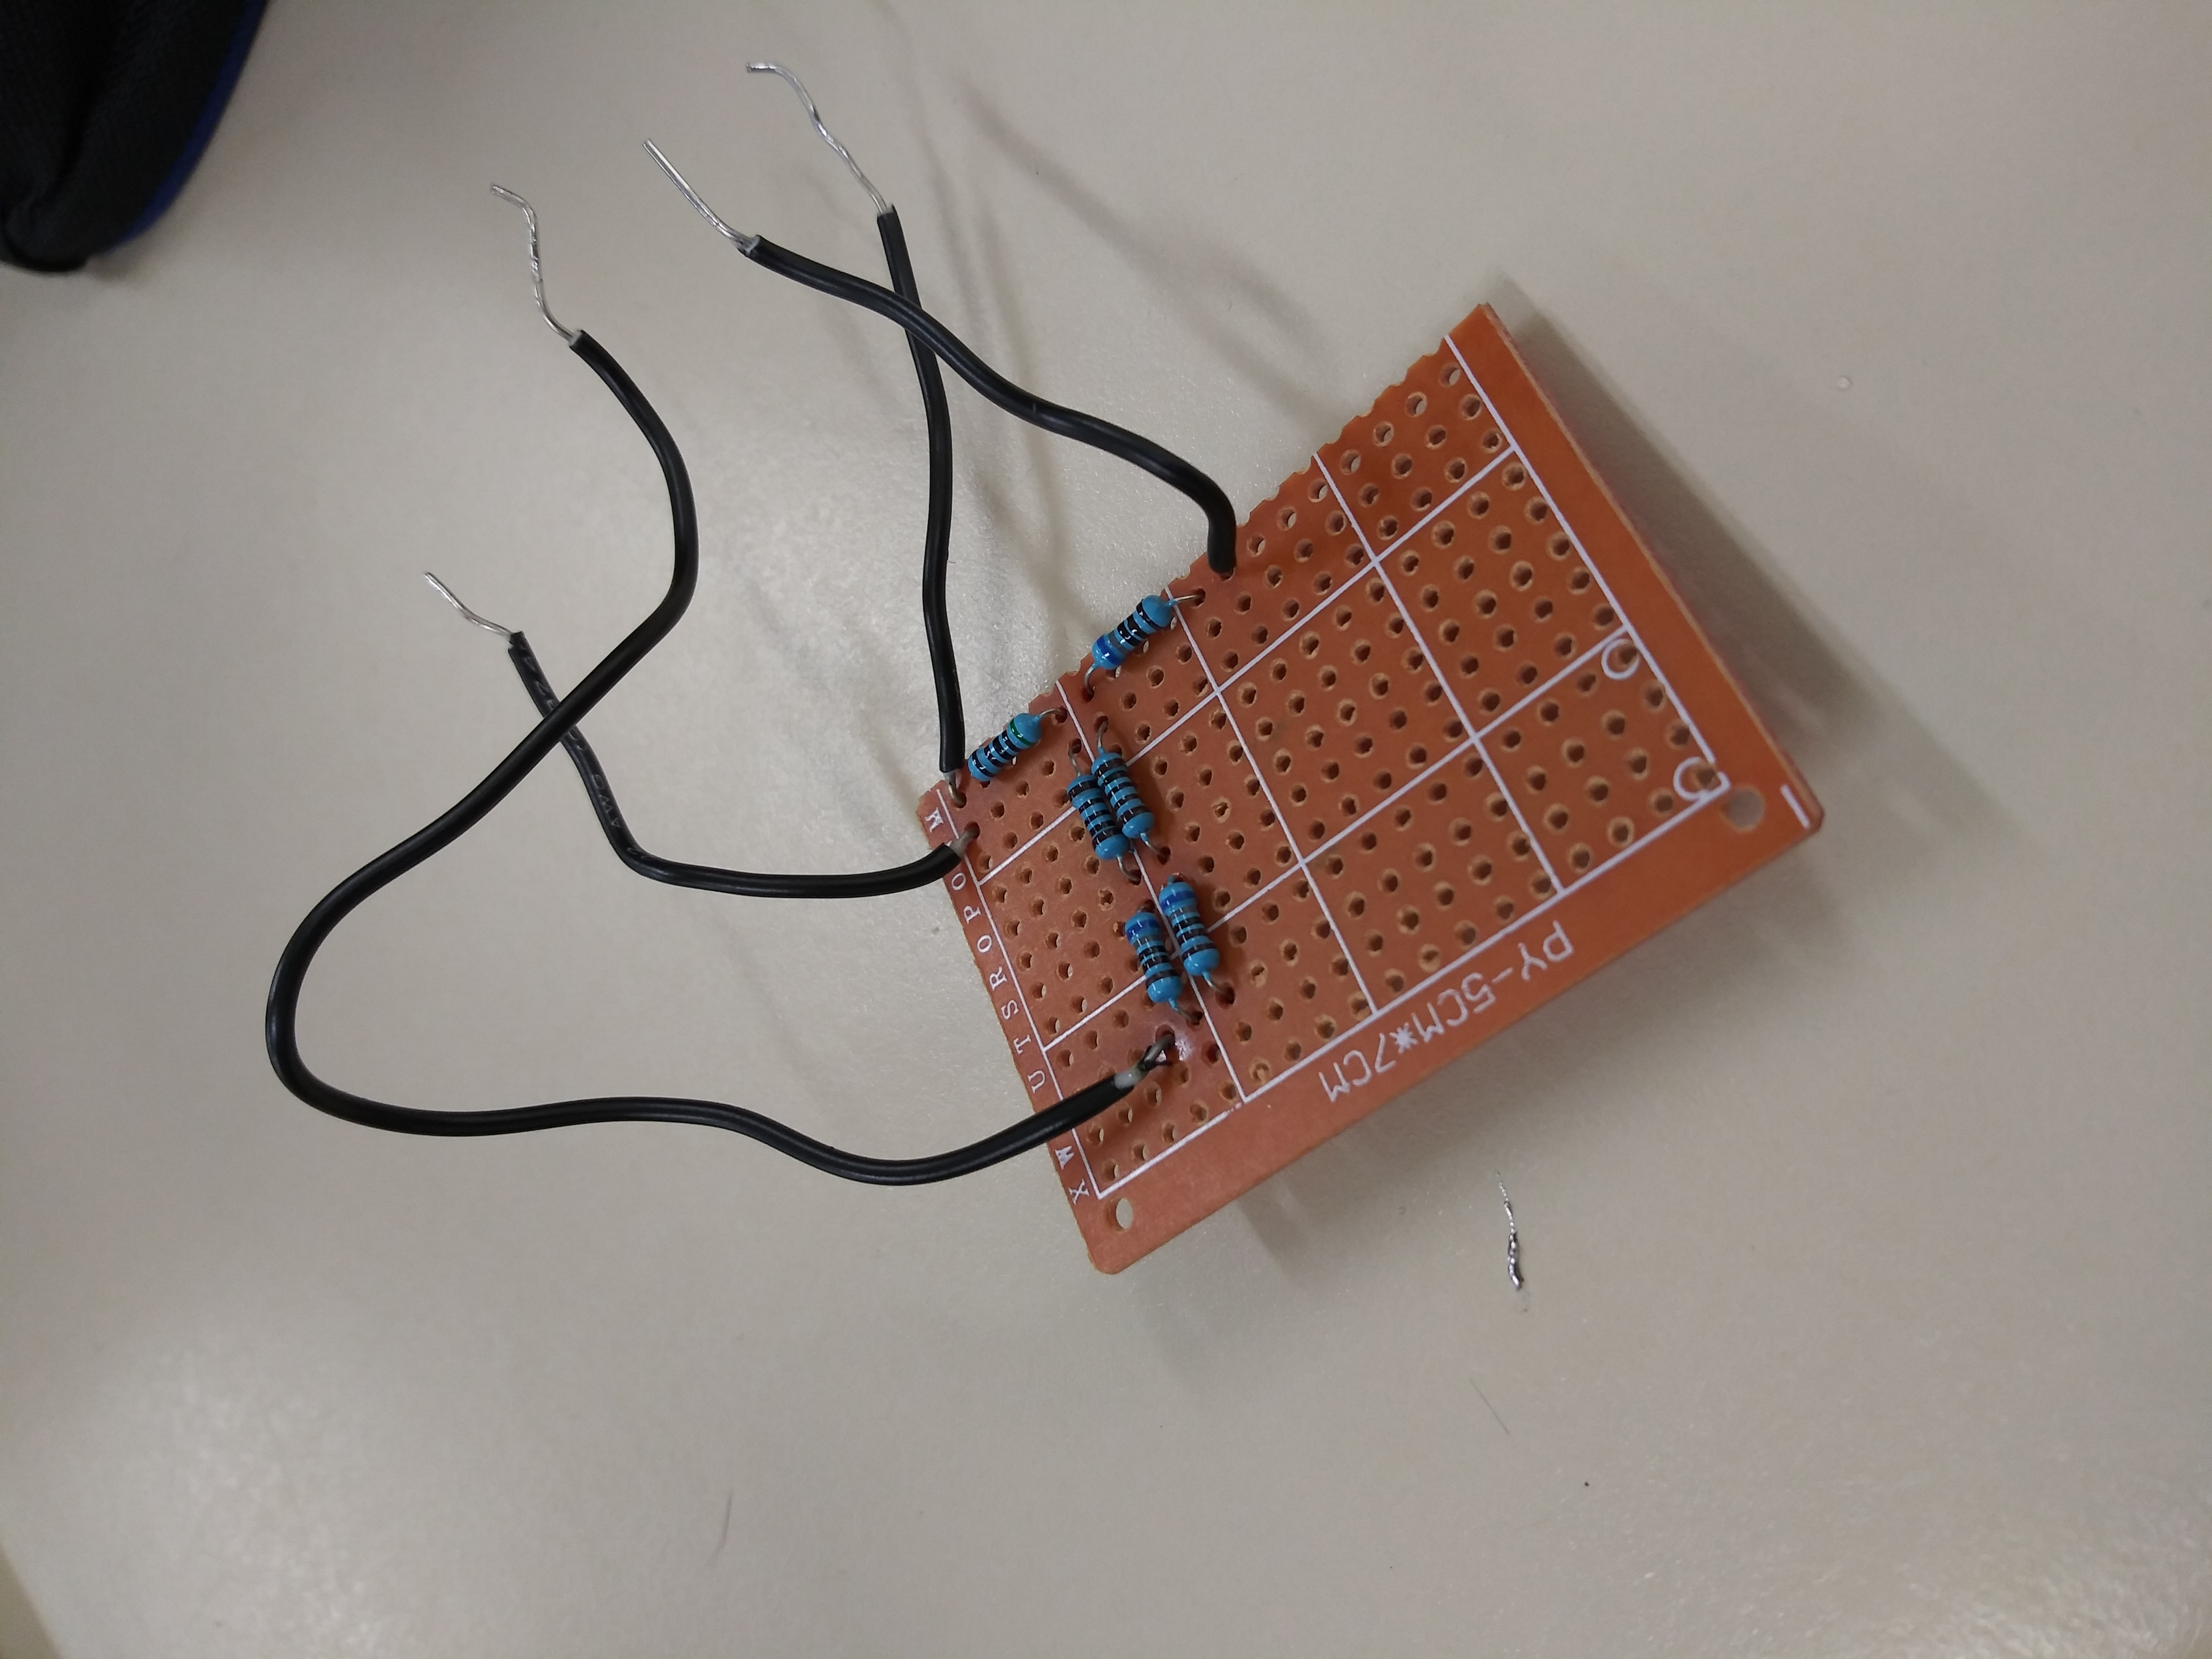
\includegraphics[width=\textwidth]{Images/20191029_142450.jpg}

The connections (from left to right) are as follows: \SI{12}{\volt}
positive, \SI{12}{V} ground, \SI{5}{V} ground, and \SI{5}{V} positive.

\end{document}

5.58
1.31
6.35

M0 = 12 V in
V3 = 12 V  ground
M9 = 5 V ground
